%% State Space Modelling of Dynamic Systems
%% Lecture 20: State Feedback Control
\def\FileDate{10/02/02}
\def\FileVersion{1.0}
% ----------------------------------------------------------------
% Notes pages *********************************************************
% ----------------------------------------------------------------

\begin{slide}
   \heading{State Feedback Control}
One of the advantages of state space models is that it is possible to apply state feedback to place the closed loop poles into any desired positions.

\textbf{State Space Design Methodology}

\begin{enumerate}
	\item Design control law to place closed loop poles where desired
	\item If full state not available for feedback, then design an \emph{Observer} to compute the states from the system output
	\item Combine \emph{Observer} and \emph{Controller} -- this takes the place of the \emph{Classical Compensator}
	\item Introduce the \emph{Reference Input} -- affects the closed loop zeros but not the poles making it possible to improve the transient response and tracking accuracy
\end{enumerate}	
\end{slide}

\begin{slide}
   \heading{State Feedback Compensator}
   \begin{center}
   	\resizebox{280pt}{!}{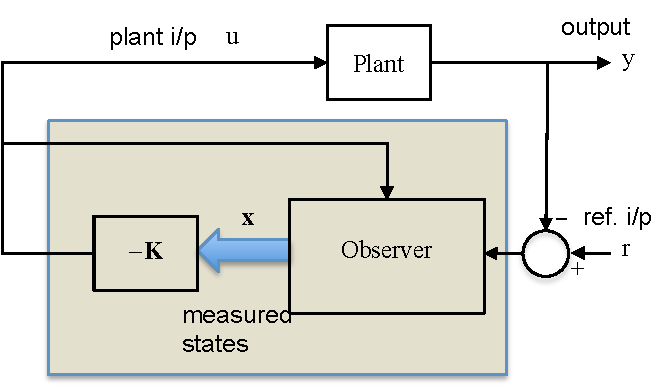
\includegraphics{pictures/statefb.pdf}}
   \end{center}
\end{slide}

\section*{Finding the Control Law} % (fold)
\label{sec:finding_the_control_law}

We shall only consider SISO systems here.


\begin{center}
	\resizebox{200pt}{!}{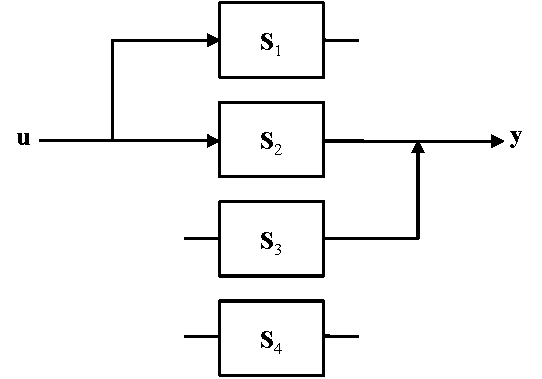
\includegraphics{pictures/partitioning.pdf}}
\end{center}
\endinput

%%% Local Variables: 
%%% mode: latex
%%% TeX-master: "notes"
%%% End:
\ifslidesonly
\begin{slide}
   \heading{Finding the Control Law (1)}
   
\begin{center}
	\resizebox{200pt}{!}{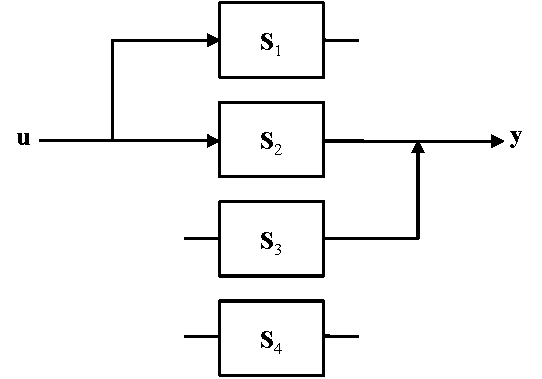
\includegraphics{pictures/partitioning.pdf}}
\end{center}
\endinput

%%% Local Variables: 
%%% mode: latex
%%% TeX-master: "notes"
%%% End:
\end{slide}
\fi

Given the transformation $\mathbf{T}^{-1}\mathbf{AT}=\mathbf{\Lambda}$:
\begin{eqnarray*}
	\mathbf{A}t & = & (\mathbf{T\Lambda T}^{-1}) t \\
	\mathbf{A}^nt^n & = & (\mathbf{T\Lambda T}^{-1})(\mathbf{T\Lambda T}^{-1})\ldots(\mathbf{T\Lambda T}^{-1})t^n \\
	                & = & \mathbf{T\Lambda T}^{-1}\mathbf{T\Lambda T}^{-1}\ldots\mathbf{T\Lambda T}^{-1}t^n \\
	\mathbf{A}^nt^n & = & \mathbf{T\Lambda}\mathbf{I}\mathbf{\Lambda I}\ldots\mathbf{I\Lambda T}^{-1}t^n \\
	\               & = & \mathbf{T\Lambda}^n\mathbf{T}^{-1}t^n \\
\end{eqnarray*}
\endinput

%%% Local Variables: 
%%% mode: latex
%%% TeX-master: "notes"
%%% End:
\ifslidesonly
\begin{slide}
	\heading{Finding the Control Law (2)}
   Given the transformation $\mathbf{T}^{-1}\mathbf{AT}=\mathbf{\Lambda}$:
\begin{eqnarray*}
	\mathbf{A}t & = & (\mathbf{T\Lambda T}^{-1}) t \\
	\mathbf{A}^nt^n & = & (\mathbf{T\Lambda T}^{-1})(\mathbf{T\Lambda T}^{-1})\ldots(\mathbf{T\Lambda T}^{-1})t^n \\
	                & = & \mathbf{T\Lambda T}^{-1}\mathbf{T\Lambda T}^{-1}\ldots\mathbf{T\Lambda T}^{-1}t^n \\
	\mathbf{A}^nt^n & = & \mathbf{T\Lambda}\mathbf{I}\mathbf{\Lambda I}\ldots\mathbf{I\Lambda T}^{-1}t^n \\
	\               & = & \mathbf{T\Lambda}^n\mathbf{T}^{-1}t^n \\
\end{eqnarray*}
\endinput

%%% Local Variables: 
%%% mode: latex
%%% TeX-master: "notes"
%%% End:
\end{slide}
\fi

 
The matrix function becomes:
\begin{eqnarray*}
	f(\mathbf{A}t) & = & f_0\mathbf{TIT}^{-1} + f_1\mathbf{T\Lambda T}^{-1}t + f_2\mathbf{T\Lambda}^2\mathbf{T}^{-1}t^2 + \cdots + f_n\mathbf{T\Lambda}^n\mathbf{T}^{-1}t^n + \cdots \\
	f(\mathbf{A}t) & = & \mathbf{T}\left(f_0\mathbf{I} + f_1\mathbf{\Lambda}t + f_2\mathbf{\Lambda}^2t^2 + \cdots + f_n\mathbf{\Lambda}^nt^n + \cdots \right)\mathbf{T}^{-1}\\
	               & = & \mathbf{T}f(\mathbf{\Lambda}t)\mathbf{T}^{-1}
\end{eqnarray*}
 
The term inside the brackets on the rhs is a diagonal matrix and the $i^\mathrm{th}$ diagonal element is:
\[
f_0+f_1\lambda_it + f_2\lambda_i^2t^2 + \cdots + f_n\lambda_i^nt^ + \cdots
\]
From the Taylor series this must be $f(\lambda_i t)$:
\[
f(\mathbf{A} t)=\mathbf{T} f(\mathbf{\Lambda} t) \mathbf{T}^{-1}
\]   
where $f(\mathbf{\Lambda} t)=\mathrm{diag}\left(f(\lambda_i t)\right)$.

\endinput

%%% Local Variables: 
%%% mode: latex
%%% TeX-master: "notes"
%%% End:
\ifslidesonly
\begin{slide}
	\heading{Finding the Control Law (3)}
   The matrix function becomes:
\begin{eqnarray*}
	f(\mathbf{A}t) & = & f_0\mathbf{TIT}^{-1} + f_1\mathbf{T\Lambda T}^{-1}t + f_2\mathbf{T\Lambda}^2\mathbf{T}^{-1}t^2 + \cdots + f_n\mathbf{T\Lambda}^n\mathbf{T}^{-1}t^n + \cdots \\
	f(\mathbf{A}t) & = & \mathbf{T}\left(f_0\mathbf{I} + f_1\mathbf{\Lambda}t + f_2\mathbf{\Lambda}^2t^2 + \cdots + f_n\mathbf{\Lambda}^nt^n + \cdots \right)\mathbf{T}^{-1}\\
	               & = & \mathbf{T}f(\mathbf{\Lambda}t)\mathbf{T}^{-1}
\end{eqnarray*}
 
The term inside the brackets on the rhs is a diagonal matrix and the $i^\mathrm{th}$ diagonal element is:
\[
f_0+f_1\lambda_it + f_2\lambda_i^2t^2 + \cdots + f_n\lambda_i^nt^ + \cdots
\]
From the Taylor series this must be $f(\lambda_i t)$:
\[
f(\mathbf{A} t)=\mathbf{T} f(\mathbf{\Lambda} t) \mathbf{T}^{-1}
\]   
where $f(\mathbf{\Lambda} t)=\mathrm{diag}\left(f(\lambda_i t)\right)$.

\endinput

%%% Local Variables: 
%%% mode: latex
%%% TeX-master: "notes"
%%% End:
\end{slide}
\fi

The vector $[v_{31}, i_{1}]^T$ is called the ``\emph{state
vector}.'' Its elements are state variables.
\endinput
%%% Local Variables: 
%%% mode: latex
%%% TeX-master: "notes"
%%% End: 

\ifslidesonly
\begin{slide}
	\heading{Finding the Control Law (4)}
   The vector $[v_{31}, i_{1}]^T$ is called the ``\emph{state
vector}.'' Its elements are state variables.
\endinput
%%% Local Variables: 
%%% mode: latex
%%% TeX-master: "notes"
%%% End: 

\end{slide}
\fi



\subsection*{Example 1} % (fold)
\label{sub:example_1}

\textbf{Problem}: Given,
\[
{\bf{\dot x}} = \left[ {\begin{array}{*{20}c}
   { - 4} & 0  \\
   0 & { - 11}  \\
\end{array}} \right]{\bf{x}} + \left[ {\begin{array}{*{20}c}
   1  \\
   { - 1}  \\
\end{array}} \right]u
\]
find the feedback control law which places the closed-loop poles at: $-10\pm j10$.

\textbf{SOLUTION}:
\begin{eqnarray*}
	0 & = & \det \left[ {s{\bf{I}} - {\bf{A}} + {\bf{BK}}} \right] = \det \left\{ {\left. {\left[ {\begin{array}{*{20}c}
	   {s + 4} & 0  \\
	   0 & {s + 11}  \\
	\end{array}} \right] + \left[ {\begin{array}{*{20}c}
	   1  \\
	   { - 1}  \\
	\end{array}} \right]\left[ {\begin{array}{*{20}c}
	   {k_1 } & {k_2 }  \\
	\end{array}} \right]} \right\}} \right. \\
	0 & = & \det \left[ {\begin{array}{*{20}c}
	   {s + 4 + k_1 } & {k_2 }  \\
	   { - k_1 } & {s + 11 - k_2 }  \\
	\end{array}} \right] \\
	0 & = & (s + 4 + k_1 )(s + 11 - k_2 ) - (k_2 )( - k_1 ) \\
	0 & = & (s+4+k_1)(s+11-k_2)+k_1k_2
\end{eqnarray*}
\begin{equation}
	\label{eq:3}
	s^2+(15+k_1-k_2)s+(44+11k_1-4k_2)=0
\end{equation}

Now the desired CE is:
\[
\alpha_c(s)=(s+10-j10)(s+10+j10) = 0
\]
\begin{equation}\label{eq:4}
	s^2+20s+200=0
\end{equation}

Therefore matching coefficients in Eqs. (\ref{eq:3}) and (\ref{eq:4}):
\[
\begin{array}{c}
 s^2 :1 = 1 \to {\rm{OK}} \\ 
 s^1 :15 + k_1  - k_2  = 20 \to k_1  - k_2  = 5 \\ 
 s^0 :44 + 11k_1  - 4k_2  = 200 \to 11k_1  - 4k_2  = 156 \\ 
 \end{array}
\]

 

Solving for the $k$'s:
\[
\left[ {\begin{array}{*{20}c}
   1 & { - 1}  \\
   {11} & { - 4}  \\
\end{array}} \right]\left[ {\begin{array}{*{20}c}
   {k_1 }  \\
   {k_2 }  \\
\end{array}} \right] = \left[ {\begin{array}{*{20}c}
   5  \\
   {156}  \\
\end{array}} \right]
\]
% MathType!MTEF!2!1!+-
% faaagaart1ev2aaaKnaaaaWenf2ys9wBH5garuavP1wzZbqedmvETj
% 2BSbqefm0B1jxALjharqqtubsr4rNCHbGeaGqiVu0Je9sqqrpepC0x
% bbL8FesqqrFfpeea0xe9Lq-Jc9vqaqpepm0xbba9pwe9Q8fs0-yqaq
% pepae9pg0FirpepeKkFr0xfr-xfr-xb9Gqpi0dc9adbaqaaeGaciGa
% aiaabeqaamaabaabaaGcbaWaamWaaeaafaWabeGabaaabaGaam4Aam
% aaBaaaleaacaaIXaaabeaaaOqaaiaadUgadaWgaaWcbaGaaGOmaaqa
% baaaaaGccaGLBbGaayzxaaGaeyypa0ZaaSaaaeaacaaIXaaabaGaey
% OeI0IaaGinaiabgUcaRiaaigdacaaIXaaaamaadmaabaqbamqabiGa
% aaqaaiabgkHiTiaaisdaaeaacaaIXaaabaGaeyOeI0IaaGymaiaaig
% daaeaacaaIXaaaaaGaay5waiaaw2faamaadmaabaqbamqabiqaaaqa
% aiaaiwdaaeaacaaIXaGaaGynaiaaiAdaaaaacaGLBbGaayzxaaGaey
% ypa0ZaaSaaaeaacaaIXaaabaGaaG4naaaadaWadaqaauaadeqaceaa
% aeaacaaIXaGaaG4maiaaiAdaaeaacaaIXaGaaGimaiaaigdaaaaaca
% GLBbGaayzxaaGaeyypa0ZaamWaaeaafaWabeGabaaabaGaaGymaiaa
% iMdacaGGUaGaaGinaiaaiMdacaaIYaGaaGyoaaqaaiaaigdacaaI0a
% GaaiOlaiaaisdacaaIYaGaaGyoaaaaaiaawUfacaGLDbaaaaa!5BC6!
\[
\left[ {\begin{array}{*{20}c}
   {k_1 }  \\
   {k_2 }  \\
\end{array}} \right] = \frac{1}{{ - 4 + 11}}\left[ {\begin{array}{*{20}c}
   { - 4} & 1  \\
   { - 11} & 1  \\
\end{array}} \right]\left[ {\begin{array}{*{20}c}
   5  \\
   {156}  \\
\end{array}} \right] = \frac{1}{7}\left[ {\begin{array}{*{20}c}
   {136}  \\
   {101}  \\
\end{array}} \right] = \left[ {\begin{array}{*{20}c}
   {19.429}  \\
   {14.429}  \\
\end{array}} \right]
\]

 

Therefore the required feedback control law is:
% MathType!MTEF!2!1!+-
% faaagaart1ev2aaaKnaaaaWenf2ys9wBH5garuavP1wzZbqedmvETj
% 2BSbqefm0B1jxALjharqqtubsr4rNCHbGeaGqiVu0Je9sqqrpepC0x
% bbL8FesqqrFfpeea0xe9Lq-Jc9vqaqpepm0xbba9pwe9Q8fs0-yqaq
% pepae9pg0FirpepeKkFr0xfr-xfr-xb9Gqpi0dc9adbaqaaeGaciGa
% aiaabeqaamaabaabaaGcbaGaamyDaiabg2da9iaadkhacqGHsislda
% WadaqaauaadeqabiaaaeaacaaIXaGaaGyoaiaac6cacaaI0aGaaGOm
% aiaaiMdaaeaacaaIXaGaaGinaiaac6cacaaI0aGaaGOmaiaaiMdaaa
% aacaGLBbGaayzxaaGaaCiEaaaa!3DCD!
\[
u = r - \left[ {\begin{array}{*{20}c}
   {19.429} & {14.429}  \\
\end{array}} \right]{\bf{x}}
\]



\textbf{COMMENT}
This matching of coefficients can always be done, though it is tedious for $n>3$, \textbf{EXCEPT} in the case of the \emph{Control Canonical Form}.

% subsection example_1 (end)
 
% section finding_the_control_law (end)

\section*{State Feedback in the Case of the Control Canonical Form} % (fold)
\label{sec:state_feedback_in_the_case_of_the_control_canonical_form}


From previous work the error dynamics are:
\[
\dot{\mathbf{e}} = (\mathbf{A}-\mathbf{LC})\mathbf{e}
\]
Therefore the dynamics of the combined system is:
\[\left[ {\begin{array}{*{20}c}
   {\dot{\mathbf{x}}}  \\
   {\dot{\mathbf{e}}ß}  \\
\end{array}} \right] = \left[ {\begin{array}{*{20}c}
   {\left( {{\bf{A}} - {\bf{BK}}} \right)} & {{\bf{BK}}}  \\
   {\bf{0}} & {\left( {{\bf{A}} - {\bf{LC}}} \right)}  \\
\end{array}} \right]\left[ {\begin{array}{*{20}c}
   {\bf{x}}  \\
   {\bf{e}}  \\
\end{array}} \right] + \left[ {\begin{array}{*{20}c}
   {\bf{B}}  \\
   {\bf{0}}  \\
\end{array}} \right]r
\]
\endinput

%%% Local Variables: 
%%% mode: latex
%%% TeX-master: "notes"
%%% End:
\ifslidesonly
\begin{slide}
	\heading{Control Canonical Form Simplifies Calculation (1)}
   From previous work the error dynamics are:
\[
\dot{\mathbf{e}} = (\mathbf{A}-\mathbf{LC})\mathbf{e}
\]
Therefore the dynamics of the combined system is:
\[\left[ {\begin{array}{*{20}c}
   {\dot{\mathbf{x}}}  \\
   {\dot{\mathbf{e}}ß}  \\
\end{array}} \right] = \left[ {\begin{array}{*{20}c}
   {\left( {{\bf{A}} - {\bf{BK}}} \right)} & {{\bf{BK}}}  \\
   {\bf{0}} & {\left( {{\bf{A}} - {\bf{LC}}} \right)}  \\
\end{array}} \right]\left[ {\begin{array}{*{20}c}
   {\bf{x}}  \\
   {\bf{e}}  \\
\end{array}} \right] + \left[ {\begin{array}{*{20}c}
   {\bf{B}}  \\
   {\bf{0}}  \\
\end{array}} \right]r
\]
\endinput

%%% Local Variables: 
%%% mode: latex
%%% TeX-master: "notes"
%%% End:
\end{slide}
\fi


When the initial conditions of the state-variables are all zero,
this reduces to the transfer matrix model
\begin{equation}\label{eqn:transfer-function}
  \mathbf{Y}=\left[\mathbf{C}\left[s\mathbf{I}-\mathbf{A}\right]^{-1}\mathbf{B}+\mathbf{D}\right]\mathbf{U}
\end{equation}

\endinput

%%% Local Variables: 
%%% mode: latex
%%% TeX-master: "notes"
%%% End: 

When the observer canonical form is not used, then the design of the observer is more difficult. Ackermann's formula can be adapted as follows:
% MathType!MTEF!2!1!+-
% faaagaart1ev2aaaKnaaaaWenf2ys9wBH5garuavP1wzZbqedmvETj
% 2BSbqefm0B1jxALjharqqtubsr4rNCHbGeaGqiVu0Je9sqqrpepC0x
% bbL8FesqqrFfpeea0xe9Lq-Jc9vqaqpepm0xbba9pwe9Q8fs0-yqaq
% pepae9pg0FirpepeKkFr0xfr-xfr-xb9Gqpi0dc9adbaqaaeGaciGa
% aiaabeqaamaabaabaaGcbaGaaCitamaaCaaaleqabaGaamivaaaaki
% abg2da9maadmaabaqbamqabeabaaaabaGaaGimaaqaaiablAcilbqa
% aiaaicdaaeaacaaIXaaaaaGaay5waiaaw2faaiaad+eadaahaaWcbe
% qaaiabgkHiTiaaigdaaaGccqaHXoqydaWgaaWcbaGaam4yaaqabaGc
% caGGOaGaaCyqamaaCaaaleqabaGaamivaaaakiaacMcaaaa!3EF6!
\[
{\bf{L}}^T  = \left[ {\begin{array}{*{20}c}
   0 &  \ldots  & 0 & 1  \\
\end{array}} \right]\mathcal{O}^{ - 1} \alpha _e ({\bf{A}}^T )
\]
$\mathcal{O}$ is the observability matrix:
\[
\mathcal{O}=[\mathbf{C}^T\vdots\mathbf{A}^T\mathbf{C}^T\vdots\cdots\vdots(\mathbf{A}^T)^{n-1}\mathbf{C}^T]
\]
and if $\alpha_e(s)=s^n + \alpha_1s^{n-1}+\cdots+\alpha_n$ then \[\alpha_e(\mathbf{A}^T)=(\mathbf{A}^T)^n + \alpha_1(\mathbf{A}^T)^{n-1}+\cdots+\mathbf{I}\alpha_n.\]
 

Notice that if the system is unobservable, then the matrix inverse $\mathcal{O}^{-1}$ does not exist and we cannot design an observer for this system.


 
 

\endinput

%%% Local Variables: 
%%% mode: latex
%%% TeX-master: "notes"
%%% End:
\ifslidesonly
\begin{slide}
	\heading{Control Canonical Form (2)}
   When the initial conditions of the state-variables are all zero,
this reduces to the transfer matrix model
\begin{equation}\label{eqn:transfer-function}
  \mathbf{Y}=\left[\mathbf{C}\left[s\mathbf{I}-\mathbf{A}\right]^{-1}\mathbf{B}+\mathbf{D}\right]\mathbf{U}
\end{equation}

\endinput

%%% Local Variables: 
%%% mode: latex
%%% TeX-master: "notes"
%%% End: 

\end{slide}
\begin{slide}
	\heading{Control Canonical Form (3)}
   When the observer canonical form is not used, then the design of the observer is more difficult. Ackermann's formula can be adapted as follows:
% MathType!MTEF!2!1!+-
% faaagaart1ev2aaaKnaaaaWenf2ys9wBH5garuavP1wzZbqedmvETj
% 2BSbqefm0B1jxALjharqqtubsr4rNCHbGeaGqiVu0Je9sqqrpepC0x
% bbL8FesqqrFfpeea0xe9Lq-Jc9vqaqpepm0xbba9pwe9Q8fs0-yqaq
% pepae9pg0FirpepeKkFr0xfr-xfr-xb9Gqpi0dc9adbaqaaeGaciGa
% aiaabeqaamaabaabaaGcbaGaaCitamaaCaaaleqabaGaamivaaaaki
% abg2da9maadmaabaqbamqabeabaaaabaGaaGimaaqaaiablAcilbqa
% aiaaicdaaeaacaaIXaaaaaGaay5waiaaw2faaiaad+eadaahaaWcbe
% qaaiabgkHiTiaaigdaaaGccqaHXoqydaWgaaWcbaGaam4yaaqabaGc
% caGGOaGaaCyqamaaCaaaleqabaGaamivaaaakiaacMcaaaa!3EF6!
\[
{\bf{L}}^T  = \left[ {\begin{array}{*{20}c}
   0 &  \ldots  & 0 & 1  \\
\end{array}} \right]\mathcal{O}^{ - 1} \alpha _e ({\bf{A}}^T )
\]
$\mathcal{O}$ is the observability matrix:
\[
\mathcal{O}=[\mathbf{C}^T\vdots\mathbf{A}^T\mathbf{C}^T\vdots\cdots\vdots(\mathbf{A}^T)^{n-1}\mathbf{C}^T]
\]
and if $\alpha_e(s)=s^n + \alpha_1s^{n-1}+\cdots+\alpha_n$ then \[\alpha_e(\mathbf{A}^T)=(\mathbf{A}^T)^n + \alpha_1(\mathbf{A}^T)^{n-1}+\cdots+\mathbf{I}\alpha_n.\]
 

Notice that if the system is unobservable, then the matrix inverse $\mathcal{O}^{-1}$ does not exist and we cannot design an observer for this system.


 
 

\endinput

%%% Local Variables: 
%%% mode: latex
%%% TeX-master: "notes"
%%% End:
\end{slide}
\fi


 
\begin{itemize}
	\item Rule of thumb: observer poles can be faster than the controller poles (i.e. further from the origin) by a factor of 2 to 6. This makes the effect of the observer dynamics short-term and the overall response is dominated by the controller poles.
	\item If noise/disturbance is present this has an effect on the choice:
	\begin{description}
		\item[Process noise $w$:] $d\mathbf{x}/dt=\mathbf{Ax}+\mathbf{B}u+\mathbf{B}_1 w$
		\item[Sensor noise $v$:]  $y = \mathbf{C}x+v$
		\item[Observer:] $d\hat{\mathbf{x}}=\mathbf{A}\hat{\mathbf{x}}+\mathbf{B}u+\mathbf{L}(y-\mathbf{C}\hat{\mathbf{x}})$
		\item[Error $\mathbf{e}=\mathbf{x}-\hat{\mathbf{x}}$:] $d\mathbf{e}/dt=(\mathbf{A}-\mathbf{LC})\mathbf{e}+\mathbf{B}_1 w - \mathbf{L}v.$
	\end{description}
\end{itemize}

\endinput

%%% Local Variables: 
%%% mode: latex
%%% TeX-master: "notes"
%%% End:
\ifslidesonly
\begin{slide}
	\heading{Control Canonical Form (4)}
   \begin{itemize}
	\item Rule of thumb: observer poles can be faster than the controller poles (i.e. further from the origin) by a factor of 2 to 6. This makes the effect of the observer dynamics short-term and the overall response is dominated by the controller poles.
	\item If noise/disturbance is present this has an effect on the choice:
	\begin{description}
		\item[Process noise $w$:] $d\mathbf{x}/dt=\mathbf{Ax}+\mathbf{B}u+\mathbf{B}_1 w$
		\item[Sensor noise $v$:]  $y = \mathbf{C}x+v$
		\item[Observer:] $d\hat{\mathbf{x}}=\mathbf{A}\hat{\mathbf{x}}+\mathbf{B}u+\mathbf{L}(y-\mathbf{C}\hat{\mathbf{x}})$
		\item[Error $\mathbf{e}=\mathbf{x}-\hat{\mathbf{x}}$:] $d\mathbf{e}/dt=(\mathbf{A}-\mathbf{LC})\mathbf{e}+\mathbf{B}_1 w - \mathbf{L}v.$
	\end{description}
\end{itemize}

\endinput

%%% Local Variables: 
%%% mode: latex
%%% TeX-master: "notes"
%%% End:
\end{slide}
\fi

 
\subsection*{Example 2} % (fold)
\label{sub:example_2}

\textbf{Problem}: Given the system TF:
\[
G(s) = \frac{7}{(s+4)(s+11)}
\]
find the control law for the control canonical form which places the closed loop poles at $s=−10\pm j10$.

\textbf{SOLUTION}:
\[
G(s) = \frac{7}{(s+4)(s+11)} = \frac{7}{(s^2+15s+44)}
\]
 
The control canonical form has matrices:
\[
{\bf{A}} = \left[ {\begin{array}{*{20}c}
   { - 15} & { - 44}  \\
   1 & 0  \\
\end{array}} \right];\quad {\bf{B}} = \left[ {\begin{array}{*{20}c}
   1  \\
   0  \\
\end{array}} \right];\quad {\bf{C}} = \left[ {\begin{array}{*{20}c}
   0 & 7  \\
\end{array}} \right];\quad {\bf{D}} = 0
\]
 
\textbf{NB}:  $\mathbf{C}$ is obtained from the TF numerator $(0s+7)$.
so:    
\[
{\bf{A}} - {\bf{BK}} = \left[ {\begin{array}{*{20}c}
   { - 15 - k_1 } & { - 44 - k_2 }  \\
   1 & 0  \\
\end{array}} \right]
\]
and the closed loop CE is:
\begin{equation}
	s^2+(15+k_1)s+(44+k_2)=0 \label{eq:7}
\end{equation}
The desired CE is:
\[
\alpha_c(s)=(s+10-j10)(s+10+j10) = 0
\]
\begin{equation}\label{eq:8}
	s^2+20s+200=0
\end{equation}
 
Comparing Eqs. (\ref{eq:7})  and  (\ref{eq:8}) gives:
% MathType!MTEF!2!1!+-
% faaagaart1ev2aaaKnaaaaWenf2ys9wBH5garuavP1wzZbqedmvETj
% 2BSbqefm0B1jxALjharqqtubsr4rNCHbGeaGqiVu0Je9sqqrpepC0x
% bbL8FesqqrFfpeea0xe9Lq-Jc9vqaqpepm0xbba9pwe9Q8fs0-yqaq
% pepae9pg0FirpepeKkFr0xfr-xfr-xb9Gqpi0dc9adbaqaaeGaciGa
% aiaabeqaamaabaabaaGcbaGaaGymaiaaiwdacqGHRaWkcaWGRbWaaS
% baaSqaaiaaigdaaeqaaOGaeyypa0JaaGOmaiaaicdacqGHsgIRcaWG
% RbWaaSbaaSqaaiaaigdaaeqaaOGaeyypa0JaaGynaaaa!3A5E!
\[
15 + k_1  = 20 \to k_1  = 5
\]
and
% MathType!MTEF!2!1!+-
% faaagaart1ev2aaaKnaaaaWenf2ys9wBH5garuavP1wzZbqedmvETj
% 2BSbqefm0B1jxALjharqqtubsr4rNCHbGeaGqiVu0Je9sqqrpepC0x
% bbL8FesqqrFfpeea0xe9Lq-Jc9vqaqpepm0xbba9pwe9Q8fs0-yqaq
% pepae9pg0FirpepeKkFr0xfr-xfr-xb9Gqpi0dc9adbaqaaeGaciGa
% aiaabeqaamaabaabaaGcbaGaaGymaiaaiwdacqGHRaWkcaWGRbWaaS
% baaSqaaiaaigdaaeqaaOGaeyypa0JaaGOmaiaaicdacqGHsgIRcaWG
% RbWaaSbaaSqaaiaaigdaaeqaaOGaeyypa0JaaGynaaaa!3A5E!
\[
44 + k_2  = 200 \to k_2  = 156
\]
giving the control law as:   
\[
u = r - \left[ {\begin{array}{*{20}c}
   {5} & {156}  \\
\end{array}} \right]{\bf{x}}
\]

% subsection example_2 (end)Given the system TF:


% section state_feedback_in_the_case_of_the_control_canonical_form (end)

\section*{A Transfer Function Model of State Feedback} % (fold)
\label{sec:a_transfer_function_model_of_state_feedback}

The last example had a system TF with no zeros. In this case it is easy to construct the equivalent classical controller. We had the feedback law:
\[
u=r-5x_1-156x_2
\]

Now $y=7x_2$ and $\dot{x}_2=x_1$ therefore $X_2(s)=Y(s)/7$ and $X_1(s)=sX_2(s)=sY(s)/7$. Therefore
\begin{eqnarray*}
	U(s) & = & R(s)-rX_1(s)-156X_2(s) \\
	& = & R(s) - \frac{1}{7}(5s+156)Y(s)
\end{eqnarray*}

\endinput

%%% Local Variables: 
%%% mode: latex
%%% TeX-master: "notes"
%%% End:
\ifslidesonly
\begin{slide}
	\heading{Transfer Function Model of State Feedback (1)}
   The last example had a system TF with no zeros. In this case it is easy to construct the equivalent classical controller. We had the feedback law:
\[
u=r-5x_1-156x_2
\]

Now $y=7x_2$ and $\dot{x}_2=x_1$ therefore $X_2(s)=Y(s)/7$ and $X_1(s)=sX_2(s)=sY(s)/7$. Therefore
\begin{eqnarray*}
	U(s) & = & R(s)-rX_1(s)-156X_2(s) \\
	& = & R(s) - \frac{1}{7}(5s+156)Y(s)
\end{eqnarray*}

\endinput

%%% Local Variables: 
%%% mode: latex
%%% TeX-master: "notes"
%%% End:
\end{slide}
\fi

\[
s{\bf{\hat X}}(s) =  {\bf{A\hat X}}(s) + {\bf{B}}U(s) + {\bf{L}}\left( {Y(s) - {\bf{C\hat X}}}(s) \right)
\]
then,
\[
\left( {s{\bf{I}} - {\bf{A}} + {\bf{LC}}} \right){\bf{\hat X}}(s) = {\bf{B}}U(s) + {\bf{L}}Y(s) 
\]
or,
\[
{\bf{\hat X}}(s) = {\bf{M}}^{ - 1} {\bf{B}}U(s) + {\bf{M}}^{ - 1} {\bf{L}}Y(s)
\]


\endinput

%%% Local Variables: 
%%% mode: latex
%%% TeX-master: "notes"
%%% End:
\ifslidesonly
\begin{slide}
	\heading{Transfer Function Model of State Feedback (2)}
   \[
s{\bf{\hat X}}(s) =  {\bf{A\hat X}}(s) + {\bf{B}}U(s) + {\bf{L}}\left( {Y(s) - {\bf{C\hat X}}}(s) \right)
\]
then,
\[
\left( {s{\bf{I}} - {\bf{A}} + {\bf{LC}}} \right){\bf{\hat X}}(s) = {\bf{B}}U(s) + {\bf{L}}Y(s) 
\]
or,
\[
{\bf{\hat X}}(s) = {\bf{M}}^{ - 1} {\bf{B}}U(s) + {\bf{M}}^{ - 1} {\bf{L}}Y(s)
\]


\endinput

%%% Local Variables: 
%%% mode: latex
%%% TeX-master: "notes"
%%% End:
\end{slide}
\fi



% section a_transfer_function_model_of_state_feedback (end)

%----------------------------------------------------------------
% The end of notes
% ----------------------------------------------------------------
\endinput

%%% Local Variables: 
%%% mode: latex
%%% TeX-master: t
%%% End: 
